\documentclass[12pt]{article}

% Any percent sign marks a comment to the end of the line

% Every latex document starts with a documentclass declaration like this
% The option dvips allows for graphics, 12pt is the font size, and article
%   is the style




% array/table
\usepackage{array}
\usepackage{multirow}

% figure
\usepackage[pdftex]{graphicx}
\usepackage{epsfig}
\usepackage[hang]{subfigure}
\usepackage[small,bf]{caption}
\usepackage{amsmath}
\usepackage{enumitem}
\usepackage{tabularx}
\usepackage{ctable}


\usepackage{authblk}
\renewcommand\Authands{ and }

%clickable ref
\usepackage[backref,pagebackref,naturalnames=true,colorlinks]{hyperref}



\setlength{\oddsidemargin}{0.25in}
\setlength{\textwidth}{6.5in}
\setlength{\topmargin}{0in}
\setlength{\textheight}{8.5in}



%----------------------------------------------------------------------------------------
%        DOCUMENT INFORMATION
%----------------------------------------------------------------------------------------

\title{EG01-EG23 Transition: Cyclus Results}


\author[1]{B. Mouginot\thanks{\href{mailto:mouginot@wisc.edu}{mouginot@wisc.edu}}}
\author[1]{P.P.H. Wilson \thanks{\href{mailto:paul.wilson@wisc.edu}{paul.wilson@wisc.edu}}}
\author[1]{R. Carlsen \thanks{\href{mailto:rcarlsen@wisc.edu}{rcarlsen@wisc.edu}}}
\affil[1]{University of Wisconsin--Madison, Department of Engineering Physics, CNERG group}


\date{\today}

\setlength{\parindent}{0em}
\setlength{\parskip}{0.7em}

\begin{document}
\maketitle

\section{Intro/specification}

One of the activities of the U.S. Department of Energy (DOE) Fuel Cycle Option (FCO) campaign is
to assess the future of the U.S. nuclear fleet. During the Evaluation and Screening study, 
several alternative fuel cycles were analyzed in an equilibrium state and organized into Evaluation
Groups (EG).  In the current phase the DOE has been interested in assessing a transition from the
current once-through fuel cycle to some of the best alternatives from their
equilibrium analysis.

The analysis in this report was conducted done after similar analyses performed by the
three fuel cycle simulator codes DYMOND, \cite{dymon}, VISION \cite{vision},
and ORION \cite{orion}. The purpose of this report is to demonstrate the
capabilities of the Cyclus simulator \cite{cyclus} as sufficiently mature to
contribute to ongoing fuel cycle analysis work.

\section{Scenario Description}

The scenario used in this study models the transition from a once-through
light water reactor (LWR) fuel cycle (i.e. EG01) to a 
full recycle case (i.e. EG23) with only sodium fast reactors
(SFR).  The LWR and SFR deployments were
selected to accomplish three primary goals:

\begin{itemize}
    \item Follow the 1\% annual electricity production curve (Figure \ref{fig:nrg}).
    \item Minimize the amount of sitting separated plutonium.
    \item Transition as quickly as possible given the other goals.
\end{itemize}

The rector deployment schedule (Figure \ref{fig:deploy}) is part of the problem
specification. It has been taken from a DYMOND calculation by B. Feng\cite{B.Feng_calculation} 
and implemented in
Cyclus (with some approximation which will be detailed further in the
document).

Other scenario details, including how to represent the problem specifications in Cyclus,
are based on previous work done by R. Carlsen
(https://github.com/rwcarlsen/eg23-sim).  From this study, the configuration
and deployment schedule of the separation facilities for LWR used fuel have
been taken.

\begin{figure}[h!]
    \centering
    \subfigure[Deployment schedule\label{fig:deploy}]  {\epsfig{figure=img/CapacityStarted,width=0.48\textwidth}}
    \subfigure[Electricity produced\label{fig:nrg}]    {\epsfig{figure=img/ElectricityGenerated,width=0.48\textwidth}}
    \caption{
        Deployment schedule and corresponding electricity produced by the
        different reactors where R1(blue): existing LWR, R2(green): new
        builded LWR, R3(red): high SFR, R4(purple): low
        SFR.\label{fig:deployment}
    }
\end{figure}

By default, Cyclus facilities exhibit greedy behavior: they request and
process as much material as they can given their inventory capacities and
process throughput limits. As Cyclus does not yet include direct support for on-demand
processing, some special accommodations were made to maintain the desired low
inventory of separated Pu. In order to address this in parts, a series of two
simulations were run:

\begin{itemize}

    \item \textbf{Case 1}: A simulation with fuel fabrication deployments
        matching capacity for SFR fresh fuel demand over time, but with
        unrestricted, greedy spent fuel separations.

    \item \textbf{Case 2}: A simulation with separations throughput changing
        over time. Results from the first simulation were used to calculate
        the required separations deployments over time in order to approximate
        on-demand separations.

\end{itemize}

Scenario details for cases 1 and 2 are identical except for the changes noted in
Section \ref{sec:case2}.

The following subsections describe the configuration of the primary facility
types (i.e. Cyclus prototypes) used in this analysis.

\subsection{Reactors}

After the LWR to SFR transition is completed, new SFR reactors are deployed
with a lower breeding ratio in order to prevent unbounded buildup of
plutonium. The properties of the different reactors cores used for the
simulation have been summarized in Table \ref{tab:reactor}. Two different SFR 
configurations exist to facilitate management of Pu in later years by reducing
the breeding ratio.  Because of the 1-month timestep of Cyclus, the batch quantity and cycle length
parameters have been manipulated to match as closely as possible important
invariants such as fuel residence time, burnup, and discharge rates
\cite{B.Feng_calculation}. The notion of batches
is defined in Cyclus by combining the number of assemblies per core and 
the number of assemblies per batch.  In the simplest form, an integer number of
batches, n, can be defined by specifying n assemblies per core and 1 assembly
per batch.  For a non-integer number of batches, f, can be implemented by
specifying f$\times 10^m$ number of assemblies per core and $10^m$ assemblies
per batch, where f$\times 10^m$ is an integer.  For this problem, it is also
possible to select the cycle length, number of batches and batch size to
approximate the same fuel throughput.  This choice implies small 
discrepencies between specifications and Cyclus input that have been detailed 
below.

\begin{table}[h!]
    \centering
    \begin{tabularx}{350pt}{lXXX}
      \hline
      Core Specifications   &  LWR             &  SFR 1            &  SFR 2            \\
      \hline
      Rated Power, [MWe]    &  1000            &  400              &  400              \\
      Thermal Efficiency    &  0.33            &  0.4              &  0.4              \\
      Capacity Factor       &  0.90            &  0.90             &  0.90             \\
      Burnup, [Gwd/tHM]     &  50              &  47.501           &  42.397           \\
      Number of batches     &  3               &  5.44             &  4.44             \\
      Cycle length, [month] &  18              &  12               &  12               \\
      Core Inventory, [tHM] &  3$\times$29.565 &  37.62            &  34.40            \\
                                                                                       \\
      \multicolumn{4}{l}{Cyclus inplementation}                                        \\ 
      \hline
      \hline
      Assembly size [kgHM]  &  14784           &  1393.33          &  1563.64          \\
      Assembly in the core  &  6               &  27               &  22               \\
      Assembly per batches  &  1               &  5                &  5                \\
      Cycle length, [month] &  9               &  12               &  12               \\
      Core Inventory, [tHM] &  6$\times$14.784 &  27$\times$1.393  &  22$\times$1.564  \\
      \hline
    \end{tabularx}
    \caption{Reactor core properties.}
    \label{tab:reactor}
\end{table}


For the SFR 1 facility type, the number of batches is specified to be $5.44$ (for
discharge burnup of 37.62 GWd/t), $5.40$ has been used (27/5). For the SFR 2, $4.4$ 
batches (22/5) have been used to approximate the 4.44 batches that were specified.

An exact match to the specified number of batches is possible, but
inefficient.  For example, SFR 1 could have been implemented with
$544~$assemblies per core and $100~$assemblies per batch, but this would
result in 20 times as many material objects being traded by the dynamic
resource exchange (DRE), and thus longer runtimes and larger output databases.


%With Cyclus' 1-month time step, the burnup resolution can be
%easly calculated as:
%\begin{equation} \Delta BU = \frac{P_{th} \times \Delta t}{M_{r}},
%\end{equation}
%\noindent where $P_{th}$ is the thermal power of the reactor, $M_{r}$ its mass in
%heavy metal, $\Delta BU$ the burnup achievable precision and $\Delta t$ the time
%step size. In this simulation the $\Delta BU$ are for the SFR 1 \& 2 respectively:
%$0.73$ and $0.79~$GWd/t.
%
%This does not affect the composition of the discharge fuel as the reactor model
%used for this analysis does not perform a burnup evolution calculation. Only the
%mass of discharged fuel is affected with a respective relative error : $0.01 \%$,
%$0.0 \%$ and $0.006 \%$.


All LWR reactors use enriched uranium fuel. The SFR used MOX fuel with
different plutonium enrichments. The input/output fuel recipes are summarized
in Table \ref{tab:reactor_fuel} taken from \cite{B.Feng_calculation}.

\begin{table}[h!]
    \centering
    \begin{tabular}{lllll}
    \hline
    \multicolumn{2}{c}{Reactor}            &  LWR [$\%w$]  &  SFR fuel 1  [$\%w$] &  SFR fuel 2  [$\%w$]  \\
    \hline
    \multirow{3}{*} {In recipe}  &  235U   &  95.8         &  0                   &  0                    \\
                                 &  238U   &  4.2          &  92.36               &  91.466               \\
                                 &  Pu     &  0            &  7.64                &  8.534                \\
    \hline
    \multirow{5}{*} {Out recipe} &  235U   &  0.8          &  0                   &  0                    \\
                                 &  238U/U &  92.68        &  85.99               &  86.025               \\
                                 &  Pu     &  1.2          &  9.02                &  9.596                \\
                                 &  MA     &  0.11         &  0.13                &  0.107                \\
                                 &  FP     &  5.21         &  4.86                &  4.272                \\
    \hline
    \end{tabular}

    \caption{
        Input/Output Fuel composition recipe for the different reactors. Note that
        for the SFR reactor fuel no isotopic distinctions have been made and U in
        SFR should be considered depleted uranium in the input recipes, the
        uranium isotopic changes in the output recipes have not been investigated
        in this work.
    }

    \label{tab:reactor_fuel}
\end{table}

\subsection{Cooling/Storage}

After irradiation, all fuel is cooled for 84 months before becoming available
for reprocessing.  The Cycamore Storage facility allows defining a minimum
residence time for each incoming material.  In order to 
differentiate between material in cooling and material available for
reprocessing as specified in the reporting requirements, 
2 storage facilities are used in series providing this explicit
distinction. One dedicated to cooling, with a residence time of 84 months,
corresponds to the output quantity ``Used Fuel in Cooling Storage'', and
one dedicated to storage until reprocessing with no minimum residence time
corresponds to the output quantity ``UNF waiting for reprocessing''.

The implementation properties of the cooling storage can be found in table \ref{tab:cooling_1} 
\begin{table}[h!]
    \centering
    \begin{tabular}{ll}
    \hline
    \multicolumn{2}{l}{Cooling Implementation}  \\
    \hline
    Residence Time [month]   &  84  \\
    \hline
    \end{tabular}
    \caption{Cooling facilities core implementation.}
    \label{tab:cooling_1}
\end{table}

\subsection{Separation}

\subsubsection{Case 1: Greedy Separations}

The LWR fuel separation is handled by three identical separation facilities,
two deployed in 2030 and one in 2040. In Case 1, the SFR separation facilities have a
very large separation capacity, in the first case, we have tried to throttle
the separation rate indirectly using the gradual fuel fabrication capacity
growth. Full fabrication facilities stop requesting separated plutonium
leading to eventual halting of spent fuel separations.
As the separation output buffers are not limited, those separation facilities will
reprocess all the used available fuel with a constant reprocessing rate.

As the fuel fabrication facilities have a tuned deployement and capacities (for 10
batchs of fuel), we are reporting for ``Fuel Resource in Storage'' is based on the
inventories of the separation facilities plutonium output buffer.
The reprocessed uranium is sent after the sepration to a dedicateed storage.

Notable are subtle differences in what these two storage facilities data represent
and their exact semantic meaning in the analysis spreadsheet.
%% NOTE: if LWR separations output buffers are unlimited, it will never stop
%% separating, right?

\begin{table}[h!]
    \centering
    \begin{tabular}{lllll}
    \hline
    Separation Implementation  &  LWR        &  SFR 1/2    \\
    \hline
    Throughput [tHM/month]     &  83.3333    &  5000       \\
    feed buffer [tHM]          &  107.537    &  5000       \\
    Pu output buffer [tHM]     &  Unlimited  &  5000       \\
    Pu separation efficiency   &  0.99       &  0.99       \\
    Recycled U buffer [tHM]    &  Unlimited  &  Unlimited  \\
    U separation efficiency    &  0.99       &  0.99       \\
    Waste buffer [tHM]         &  Unlimited  &  Unlimited  \\
    \hline
    \end{tabular}
    \caption{Separation facilities core properties. }
    \label{tab:separation_1}
\end{table}

\subsubsection{Case 2: On-Demand Separations}
\label{sec:case2}

The only difference with the Case 1 scenario is the way in which reprocessing
capacity is handled over time.  Modeling on-demand separations is approximated by
deploying many small separations facilities according to plutonium requirements
for SFR fuel fabrication.  These Pu requirements were determined from the Case 1
results. While the calculated deployment schedule does not follow plutonium usage
exactly, it is a reasonable aproximation.

For this calculation, all fuels are reprocessed by only one type of reprocessing
facility (i.e. one Cyclus prototype). The fuel input preferences have been set to
3 for all irradiated UOX fuel, 2 for higher breeding ratio SFR spent fuel, and 3
for the lower breeding ratio SFR spent fuel.  Since a higher number indicates a
higher preference, these facilities will prefer to consume and process irradiated
UOX fuel and low breeding ratio SFR fuel before they consume/process high breeding
ratio SFR fuel.  The implemented characteristics of each of the reprocessing
facilities used in Case 2 are summarized in Table
\ref{tab:fuelfab_2}.

\begin{table}[h!]
    \centering
    \begin{tabular}{ll}
    \hline
    Separation Implementation  &  All Fuel   \\
    \hline
    Throughput [tHM/month]     &  60         \\
    Feed buffer [tHM]          &  66         \\
    Pu output buffer  [tHM]    &  6          \\
    Pu separation efficiency   &  0.99       \\
    Recycled U buffer [tHM]    &  Unlimited  \\
    U separation efficiency    &  0.99       \\
    Waste buffer [tHM]         &  Unlimited  \\ 
                                             \\
    \multicolumn{2}{c}{Feed commmodities}    \\
%    \hline
    \hline
    Commodity Sources         &  Preferences \\
    LWR UOX A                 &  3           \\
    LWR UOX B                 &  3           \\
    SFR MOX A                 &  2           \\
    SFR MOX B                 &  1           \\
    \hline
    \end{tabular}
    \caption{Separation facilities implementation.}
    \label{tab:fuelfab_2}
\end{table}

The Cycamore separation facility requests the feed commodities, accordingly to the
set preferences, to fill its feed buffer. The material in the feed buffer is then
separated following the implemented separation instruction and efficiency all the
unused material is send to the waste. The reprocessing rate in limited by:

\begin{itemize}

  \item the feed buffer inventory
  \item the total throughput which limits the amount of material reprocessed from
    the feed buffer,
  \item each stream throughput which limits the amount of each stream produced,
  \item the output stream bufer size.

\end{itemize}
If one of this parameter reach its limit the separation is stopped until the
constrain is release, either by the occurance of the next timestep (for the
throughput limits), either by a change in the buffers inventories. 

\subsection{Fuel Fabrication}

The UOX fuel fabrication is handled by one enrichment facility, the properties
of this enrichment facilities are summarized in Table \ref{tab:enrich_1}. As
explain the specifcication of the enrichment facility have been taken from the
R. Carlsen calculation and might differ from the exact EG01-23 transition
specifications. 

\begin{table}[h!]
    \centering
    \begin{tabular}{lllll}
    \hline
    Enrichment implementation  &  UOX        \\
    \hline
    Throughput [tHM/month]     &  Unlimited  \\
    SWU capacity [tSWU/month]  &  Unlimited  \\
    Tails assay                &  0.0025     \\
    Feed buffer [tHM]          &  Unlimited  \\
    \hline
    \end{tabular}
    \caption{Enrichment facilities implementation. }
    \label{tab:enrich_1}
\end{table}

The Fuel fabrication of the additionnal Cycamore module mix the two
input stream accordingly to the plutonium-Equivalent theory\cite{Pueq}. A
reactivity weight is calculated for the require output composition and both of
the input stream. An interpolation is used to compute a mixing ratio of the input
streams that matches the target weight.

%% QUESTION: Does the ``are supposed to be'' mean that the problem specifies
%% this?

The SFR fuel fabrication facilities are supposed to be deployed as a rate of 1
for every 10 SFRs.  As the fuel composition and annual flux slightly change
between SFR 1 and 2, the specifications between fabrication are also slightly
different. The details of all fuel fabrication facility characteristics are
summarized in Table \ref{tab:fuelfab_1}.

\begin{table}[h!]
    \centering
    \begin{tabular}{lllll}
    \hline
    Fuel Fab Properties      &  SFR 1   &  SFR 2   \\
    \hline
    Throughput [tHM/month]   &  75.240  &  76.440  \\
    Depleted U buffer [tHM]  &  69.492  &  69.912  \\
    Pu buffer  [tHM]         &  5.748   &  5.856   \\
    \hline
    \end{tabular}
    \caption{Fuel fabrication facilities properties.}
    \label{tab:fuelfab_1}
\end{table}


\section{Results}

\subsection{Case 1: Greedy Separations}

All fuel loading metrics (Figure \ref{fig:ResourceUsed}) are the same or very
close to DYMOND simulation results. There are some observable fluctuations on the
annual fuel loading and the SWU requirements which are consistent with the
synchronized refueling cycles of the initially deployed reactors.  There are
various simple ways to stagger refueling cycles for smoother data that were not
pursued in this analysis.  Similar fluctuations apper as ``echoes'' in other
material flows later in time.

\begin{figure}[h!]
    \centering
    \subfigure[Resources Mined]          {\epsfig{figure=img/ResourceMined,width=0.48\textwidth}}
    \subfigure[SWU Requirement]           {\epsfig{figure=img/SWURequierment,width=0.48\textwidth}}
    \subfigure[Annual Fuel Loading Rate]  {\epsfig{figure=img/AnnualFuelLoading,width=0.48\textwidth}}
    \caption{Resources production and fuel loading.\label{fig:ResourceUsed} }
\end{figure}

The generated power and the deployment schedule shown in Figures
\ref{fig:deploy_sub} and \ref{fig:power_sub} match perfectly with results from the
DYMOND simulations. The time scale in the output spreadsheet filled starts in 2015
and ends in 2215, while the DYMOND calculation used as reference for the
deployment schedule ends in 2210. The sudden drop in 2210 is due to a lack of
deployment data after 2210.

%% NOTE: are we supposed to plot beyond 2210? or 2200?
%% It looks like Bo only plotted to 2210 to avoid this drop at the end... is that hard to change?

\begin{figure}[h!]
    \centering
    \subfigure[Deployment Schedule\label{fig:deploy_sub}]  {\epsfig{figure=img/CapacityStarted,width=0.48\textwidth}}
    \subfigure[Electricity Produced\label{fig:power_sub}]  {\epsfig{figure=img/ElectricityGenerated,width=0.48\textwidth}}
    \caption{Deployment schedule and corresponding
    electricity produced by the different reactors
    where R1(blue): existing LWR, R2(green): new
    builded LWR, R3(red): high SFR, R4(purple): low
    SFR.\label{fig:deployment_bis} }
\end{figure}

The other curves also appear as expected. The annual reprocessing rate (Figure
\ref{fig:reprocessing_1}) corresponds directly to the deployments. Spent UOX
reprocessing starts in 2010 with 2000 MTHM/yr with another 1000 MTHM/yr added in
2030. This reprocessing rate (UOX1 + UOX2) continues until the end of the
production of used UOX (i.e. when all LWRs are decommissioned).

\begin{figure}[h!]
    \centering
    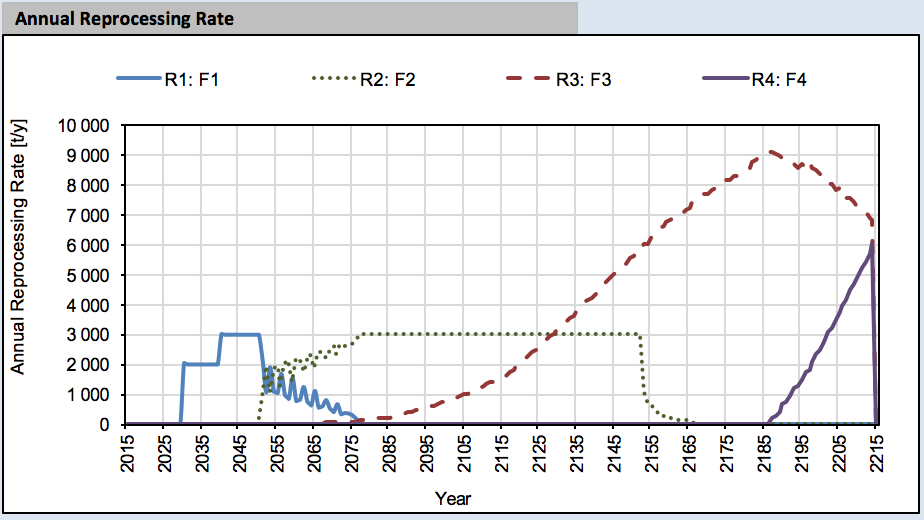
\includegraphics[width=0.62\textwidth]  {img/AnnualReprocessingRate_1}
    \caption{Annual Reprocessing Rate.}
    \label{fig:reprocessing_1}
\end{figure}


MOX spent fuel production by the 2 different SFR types roughly follows the
loading of fresh fuel.  Because the reprocessing facilities are greedy,
reprocessing all used fuel available, there is no SFR spent fuel waiting for reprocessing
because it is directly reprocessed after cooling.

\begin{figure}[h!]
    \centering
    \subfigure[Used Fuel in Cooling Storage\label{fig:UFCS_1}]  {\epsfig{figure=img/usedFuelInCooling,width=0.48\textwidth}}
    \subfigure[Fuel waiting for Reprocessing\label{fig:FWR_1}]  {\epsfig{figure=img/UNFWaitingReprocessing_1,width=0.48\textwidth}}
    \caption{Used fuel in cooling and reprocessing.\label{fig:cool_reprocc} }
\end{figure}
The amounts of the different fuels in ``Used Fuel in Cooling Storage'' (Figure
\ref{fig:UFCS_1} follow, as expected, the discharge of the different reactors.
As almost all SFR spent fuel are directly reprocessed after cooling (see Figure
\ref{fig:FWR_1}), spent fuel in storage stops increasing when all the UOX fuel has
been reprocessed. The accumulation of LWR used fuel in ``UNF Waiting for
Reprocessing'' is induced by the limited constant reprocessing capacity for those
fuel. 

\begin{figure}[h!]
    \centering
    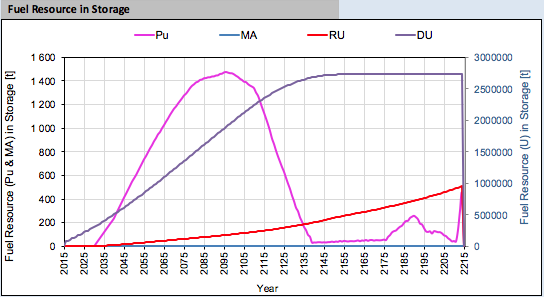
\includegraphics[width=0.62\textwidth]{img/FuelInStorage_1}
    \caption{Fuel Resource in Storage.}
    \label{fig:storagecompo_1}
\end{figure}

It appears that the capacity of the SFR fuel reprocessing is not enough to
reprocess the full inventory of MOX fuel until 2155. This explains the
appearance of MOX fuel in storage waiting for reprocessing. With the
replacement of higher breeding ratio SFRs with lower breeding ratio reactors
the MOX spent fuel generation rate decreases sufficiently for reprocessing to
"catch-up".
As shown in the Figure \ref{fig:storagecompo_1}, the reprocessing capacities of
the LWR fuel is highier than the demand on plutonium to fabricate the MOX fuel,
creating an accumulation of plutonium prior to 2100. After 2100, with the
decommision of the LWR, less LWR used fuel is produces, allowing the reduction of
the inventory of plutonium. In the other side, the reprocessing capacities of the
FBR used fuel are well adapted to the demand: the plutonium storage experience a
small accumulation just before the SFR switch of breeding ratio.
 
%As shown in the Figures \ref{fig:FC_Z} and \ref{fig:WR_Z}, the quantity of
%plutonium in storage follows the variation in the amount of MOX1 fuel in
%storage.

%\begin{figure}[h!]
%    \centering
%    \subfigure[Fuel Resource in Storage (zoomed)\label{fig:FC_Z}]       {\epsfig{figure=img/FuelInStorage_1_zoom,width=0.48\textwidth}}
%    \subfigure[Fuel waiting for reprocessing (zoomed)\label{fig:WR_Z}]  {\epsfig{figure=img/UNFWaitingReprocessing_1_zoom,width=0.48\textwidth}}
%    \caption{Plutonium in storage.\label{fig:FC_WR_zoom} }
%\end{figure}

\subsection{Case 2: On-demand Separations}

The only differences in the results between the two cases can be seen in the
behavior of the reprocessed fuel --- namely in the ``UNF fuel waiting for
reprocessing'' and in the ``Fuel Resource in Storage''.

\begin{figure}[h!]
    \centering
    \subfigure[Annual Reprocessing Rate\label{fig:ARR_2}]   {\epsfig{figure=img/AnnualReprocessingRate_2,width=0.48\textwidth}}
    \subfigure[Fuel waiting for reprocessing]               {\epsfig{figure=img/UNFWaitingReprocessing_2,width=0.48\textwidth}}
    \subfigure[Fuel Resource in Storage\label{fig:SFC_2}]  {\epsfig{figure=img/FuelInStorage_2,width=0.48\textwidth}}
    \caption{Resources production and fuel loading.\label{fig:ARR_FWR_SFC_2} }
\end{figure}

Indeed, as seen in Figure \ref{fig:ARR_2}, the reprocessing follows more closely
than in th case 1 the plutonium need of the SFR fuel fabrication. Indeed the
accumulation of plutonium is limited at $\sim500~t$ (Figure \ref{fig:SFC_2}) versus $\sim1500~t$ in the
first case. Nevertheless, one can still observe a large plutonium accumulation
spike 2100 and 2145 which one should be able to avoid with a better reprocessing
capacity deployement.

Because of both the reprocessing priority and "on-demand" separations
deployment, we observe more fuel waiting for reprocessing with a quick drop
starting around year 2090 as stored up plutonium is used in the first wave of
SFR deployments replacing aging LWRs. We can also observe some of SFR fuel
waiting for reprocessing, which decrease, showing a well designed SFR
deployment schedule that reaches an comfortable equilibrium generating
plutonium at the same rate it is being recycled.

\section{Summary}

This study has shown the capability of Cyclus to properly simulate the EG01 to
EG23 fuel cycle transition.  The main observable differences are in the
reprocessing and the storage of the used fuel, where the meaning of desired
output data (e.g. "Fuel Resource in Storage", "UNF waiting for reprocessing",
etc.) were ambiguous.  Much of the inability of Cyclus to reproduce results
from other simulators exactly can likely be attributed to this factor.

Despite Cyclus is not able now to handle exact on-demand behavior, it is
possible to deploy the different facilities with limited capacities to
"follow" material demand to mimicking an on-demand type of behavior, as shown
in Case 2.  We can also observe some small differences in the pattern of fuel
loading (and almost all the reactor fuel metrics), this comes from the way
batches are modeled discretely in Cyclus where in DYMOND all entities are
material flows are managed in a more incremental, continuous way.

%----------------------------------------------------------------------------------------
%        BIBLIOGRAPHY
%----------------------------------------------------------------------------------------

\bibliographystyle{unsrt}

\bibliography{EG23}

%----------------------------------------------------------------------------------------

\end{document}


%%% Local Variables:
%%% mode: latex
%%% TeX-master: t
%%% End:
